\subsubsection{Módulo de procesado digital}

El módulo de procesado digital es el encargado de tomar las muestras, procesarlas y generar la señal de salida. Se utiliza un \texttt{ADC} de la placa para tomar muestras a $48\ kHz$ y un \texttt{DAC} para la generación de la salida, a la misma velocidad.

\paragraph{Temporización}
\label{para:temporizacion}

La temporización de este módulo es crítica, ya que es la que garantiza la calidad de la señal procesada. 

Se utiliza un \textit{Timer} de la placa, concretamente el \texttt{TIM2} para la generación de dicha señal. Para ello, el \textit{Timer} cuenta con una señal específica de sincronización para disparar eventos de conversión, \texttt{TRGO2}. Para habilitarla, se necesita además configurar el \textit{timer} como \textit{master}, como se puede ver en el \autoref{lst:conf-tim2}. Se utiliza un valor de \textit{Prescaler} de 9 y un \textit{Period} de 224, que junto con la velocidad de reloj del sistema de 216 MHz y el divisor de APB2 de 2, provocan una velocidad final de: 

\[
    f_s = \frac{f_{CLK}}{(PRESCALER + 1)(PERIOD + 1)\cdot Div_{APB2}} = \frac{216\cdot 10^6}{(9 + 1)(224 + 1)\cdot 2} = 48\ kHz
\]

\begin{lstlisting}[captionpos=t, caption={Configuración del TRGO del \textit{timer} de sincronización}]
TIM_ClockConfigTypeDef sClockConfig = {.ClockSource = TIM_CLOCKSOURCE_INTERNAL};
if (HAL_TIM_ConfigClockSource(&htim, &sClockConfig)) {
    return -1;
}

TIM_MasterConfigTypeDef sMasterConfig = {
    .MasterOutputTrigger = TIM_TRGO_UPDATE,
    .MasterSlaveMode = TIM_MASTERSLAVEMODE_DISABLE,
};
if (HAL_TIMEx_MasterConfigSynchronization(&htim, &sMasterConfig)) {
    return -1;
}
\end{lstlisting}

Una vez configurado este timer, habrá que configurar al \texttt{ADC} y al \texttt{DAC} para que realicen las conversiones disparados por dicha señal, como se verá en los siguientes apartados.

\paragraph{Adquisición de audio}

La adquisición de audio, como ya se ha comentado, se realiza a través de un \texttt{ADC}. Los parámetros más importantes de la configuración son:
\begin{enumerate}
    \item Adquisición a través del \texttt{GPIO A6}
    \item Uso del canal 6 de muestreo
    \item Resolución de 12 bits
    \item Trigger con el \texttt{TRGO} del \texttt{TIM2}
    \item Alineación de datos a la derecha
    \item Peticiones continuas a \texttt{DMA} habilitadas
\end{enumerate}

Además, se configura el canal 0 del \textit{Stream} 4 de la \texttt{DMA2} para este \texttt{ADC}. Esto significa que se utilizará este periférico para mover las muestras constantemente del \texttt{ADC} a la memoria sin necesitar ciclos del microcontrolador, lo cual alivia seriamente la carga que recae sobre el procesador. Esta \texttt{DMA} se arranca indicándole un \textit{buffer} de memoria e informa mediante una interrupción de cuando este está a la mitad de capacidad y cuando está completamente lleno. Se configura con los siguientes parámetros:
\begin{enumerate}
    \item Dirección de periférico a memoria
    \item Incremento de dirección de periférico deshabilitado
    \item Incremento de dirección de memoria habilitada
    \item Alineación de media palabra (16 bits)
    \item Modo circular
    \item FIFO desactivada
\end{enumerate} 

Se configura incrementando solo la dirección de memoria ya que el \texttt{ADC} solo tiene una salida (por tanto no tiene sentido incrementarlo) pero interesa que se llene la zona de memoria en lugar de sustituir constantemente el mismo dato. Además, el modo circular provoca que al llegar al final del buffer se vuelva a empezar, permitiendo un flujo constante de información. Esto es muy útil como se verá en los siguientes apartados.

\paragraph{Generación de señal}

La señal la generamos a través de un \texttt{DAC} de la placa. A pesar de que no se indica en la documentación de la placa, en el \textit{datasheet} del procesador vemos que el pin \texttt{PA4} está conectado al canal 1 del \texttt{DAC}, por lo que lo utilizamos para generar la señal de salida.

La configuración más significativa de dicho periférico es:
\begin{enumerate}
    \item Uso de \texttt{GPIO PA4}
    \item Trigger a partir del \texttt{TRGO} del \texttt{TIM2}
    \item Canal 1 de salida
\end{enumerate}

Se utiliza también una \texttt{DMA} para que el \texttt{DAC} tome muestras de una zona de memoria sin necesitar que el procesador se las configure. La configuración más relevante de dicho periférico es:
\begin{enumerate}
    \item Dirección de memoria a periférico
    \item Incremento de dirección de periférico deshabilitado
    \item Incremento de dirección de memoria habilitada
    \item Alineación de media palabra (16 bits)
    \item Modo circular
    \item FIFO desactivada
\end{enumerate} 

Esta \texttt{DMA} es de dirección de periférico a memoria, pero el resto de configuración es igual y por el mismo motivo que la del ADC.

\paragraph{Sistema de Doble Buffer}

Para realizar el procesamiento de audio, la implementación más directa es utilizar un \textit{buffer} de memoria y, cuando se llene gracias al \texttt{ADC}, realizar un procesamiento de su contenido y sacarlo a través del \texttt{DAC}. Sin embargo, esto provocaría que hubiera cortes constantes mientras se procesa el audio.

Para solucionarlo, la solución más común es el uso de un mecanismo de doble \textit{buffer} o mecanismo de \textit{ping-pong}. En este algoritmo, se tienen dos \textit{buffers} de memoria (o uno con el doble de tamaño como en nuestro caso). Mientras se llena uno de los dos, se toman las muestras de el otro y se procesan. Cuando se llena por completo, se comienza a llenar el otro y se procesan las muestras del primero. \cite{PingPongBuffer}

Para nuestro caso, necesitamos realizar esta construcción dos veces, una para el \texttt{ADC} y otra para el \texttt{DAC}. Por tanto, mientras una mitad se va llenando de muestras en un lado y reproduciendo en el otro, la otra mitad del \textit{buffer} del \texttt{ADC} se procesa y se coloca el resultado en la otra mitad del \texttt{DAC}.

\begin{figure}[h]
    \centering
    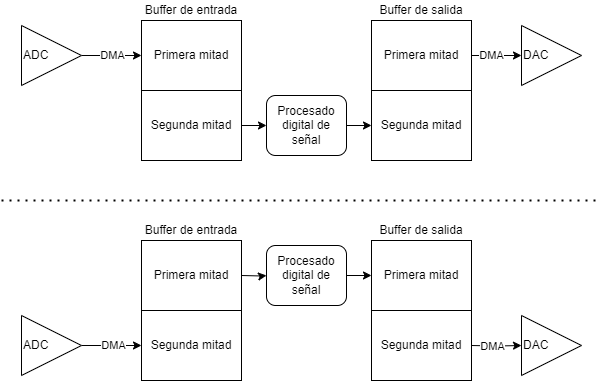
\includegraphics[width=0.5\textwidth]{images/3/3-2/DSP/doubleBuffer.png}
    \caption{Mecanismo de doble \textit{buffer} para audio}
    \label{fig:double-buffer}
\end{figure}

Este mecanismo nos permite reducir la carga del procesador sin perder calidad ni tener cortes notables en el audio.

Para implementarlo, se tiene un hilo de procesado de datos que está constantemente esperando a un par de \textit{flags} que se activan cuando se produce alguna de las interrupciones del \texttt{DMA} del \texttt{ADC}. Cuando estas se producen, se comprueba cual ha sido y se procesa la zona de memoria que corresponda.

\paragraph{Sistema de representación de coma fija}

Para el procesado de señal hemos utilizado la librería CMSIS DSP, la cual abstrae el procesamiento de señales y las matemáticas con muchos números en los procesadores de aquitectura ARM. \cite{CMSISDSPSoftware}

Para optimizarlo, permite la utilización de instrucciones \texttt{SIMD} las cuales realizan el mismo cálculo con muchos datos en un solo ciclo de reloj. Esto permite agilizar significativamente el procesado de grandes zonas de memoria, como pueden ser señales o vectores.

El principal problema de la librería son los formatos de representación con los que trabaja. No permite la utilización de números enteros normales, sino que obliga a utilizar números en coma flotante (más lentos y menos precisos) o en coma fija.

Para los números en coma fija, ARM utiliza el formato de representación de números \texttt{Q}. En este formato, los números se denotan como \texttt{QX.Y}, donde \texttt{X} es el número de bits que representan la parte entera y \texttt{Y} los bits que son parte decimal. Además, hay que indicar si el número es con signo o sin signo, si fuera con signo habría que añadir un bit que depende de la notación se debería incluir en la \texttt{X} o no (en el caso de ARM, la \texttt{X} sí incluye el bit de signo). Para manejar los números negativos se utiliza el complemento a dos.\cite{NumberFormat}

Concretamente en esta librería, se fija la parte entera a 1 bit (el de signo), por lo que el rango de números representables es aproximadamente $[-1, 1)$. Además, como siempre se utiliza el mismo número, directamente se omite, dando lugar a nombres como \texttt{Q31}, un número de 32 bits en los que el primero es el signo y los demás son parte decimal. % chktex 9

Resumiendo, en esta librería un número $x$ donde $b_n$ es el n-simo bit de menor peso, representado en \texttt{QN} es realmente:
\[ x = -b_{N} + \sum_{i = 0}^{N - 1} b_i\cdot 2^{i-N} \]

Se puede ver que este formato de representación es equivalente a dividir el formato de representación binario entre 2 elevado a el número de bits menos uno, que coincide con la $N$ del formato:

\[ x_{QN} = \frac{x_{bin}}{2^N} = \frac{-2^N\cdot b_N + \sum_{i=0}^{N - 1} b_i\cdot 2^i}{2^N} = -b_{N} + \sum_{i = 0}^{N - 1} b_i\cdot 2^{i-N} \]

Por tanto, se tiene un isomorfismo entre los dos formatos de representación que además es una operación lineal. Por tanto, todas las operaciones lineales se comportan bien con dicho isomorfismo, es decir, si se pasa un número de un formato a otro, se realiza una operación y se devuelve, es equivalente a hacer la operación en el formato original. Esto es así para las operaciones lineales que nos interesan, es decir, suma y multiplicación por una constante.

Como esas dos operaciones funcionan correctamente, se pueden realizar las siguientes operaciones utilizando números enteros de \texttt{N} bits como si fueran \texttt{QN}:
\begin{enumerate}
    \item Suma de números
    \item Producto de números
    \item Desplazamiento de números mientras no haya overflow (realmente equivalente a producto por potencia de dos)
    \item Convolución, al ser básicamente una suma ponderada
    \item Aplicación de filtro lineal, al poder reducirse a una convolución por la respuesta al impulso del filtro
\end{enumerate}

Por tanto, y como conclusión, se pueden utilizar las muestras de 12 bits del \texttt{ADC} que están almacenadas como números enteros de 16 bits como números \texttt{Q15} sin problema, por lo que la librería es ideal para nuestra aplicación. 

Para realizar pruebas y comprobar las propiedades de este formato de representación hemos utilizado una calculadora online que permite trabajar con números enteros, en coma fija y sus representaciones binarias. \footnote{\url{https://chummersone.github.io/qformat.html}}

\paragraph{Procesado Digital de la Señal}

Para el procesado de la señal, necesitamos un sistema que aplique ecualización de cinco bandas y permita ajustar el volumen del sistema. 

La ecualización se realiza mediante filtros bicuadrados, los cuales se caracterizan por configurarse con seis coeficientes: $(a_0, a_1, a_2, b_0, b_1, b_2)$. Con estos seis coeficientes se construye su función de transferencia discreta en el dominio de la transformada z:

\[ H(z) = \frac{b_0 + b_1\cdot z^{-1} + b_2\cdot z^{-2}}{a_0 + a_1\cdot z^{-1} + a_2\cdot z^{-2}}\]

Mediante filtros de esta forma se construyen filtros de tipo \textit{Peak EQ} o \textit{Shelf EQ}, los cuales incrementan o decrementan una banda de frecuencias dejando el resto sin alterar. La utilización de cinco de estos filtros en cascada permite la construcción de un ecualizador de cinco bandas. Para el cálculo de los coeficientes, hemos utilizado los que ofrece la propia librería en su documentación de referencia, específicamente para una aplicación equivalente a esta. \cite{GraphicAudioEqualizer}

Los coeficientes que ofrecen están en formato \texttt{Q31}, por lo que necesitamos utilizar filtros de dicha longitud. Esto no es un problema e incluso mejora la precisión intermedia de los cálculos. 

En CMSIS DSP, se utilizan filtros del tipo \texttt{arm\_biquad\_cas\_df1\_32x64\_q31} para los primeros dos filtros para tener más precisión en las bajas frecuencias y otros de tipo \texttt{arm\_biquad\_cascade\_df1\_q31} para el resto. Esto implica que cada banda cuenta realmente con dos etapas de filtros en cascada. Además, se fija el valor del coeficiente $a_0$ a $1$ para simplificar las cuentas. 

Por tanto, cada etapa necesita diez coeficientes en formato \texttt{q31} para su inicialización. Además, cada etapa necesita almacenar las variables de estado que se generan en cada iteración y que sirven para calcular la siguiente, por lo que se necesitan dos arrays de 8 elementos de tipo \texttt{q63} y tres arrays de 8 elementos de tipo \texttt{q31} adicionales.

Además, se necesitarán convertir las muestras de números \texttt{q15} a \texttt{q31} para realizar los cálculos, por lo que se tiene que crear un buffer intermedio del mismo tamaño que el de elementos a procesar.

La gestión de coeficientes es estática, es decir, no se puede cambiar un filtro una vez inicializado. Por ello, cuando se quiere cambiar la amplitud de una banda se necesita reinicializar el filtro. 

En total, se tienen diez coeficientes por banda y ganancia, cinco bandas y diecinueve valores posibles de ganancia por banda (desde -9 hasta 9 dB), por lo que se requieren 950 coeficientes distintos.

Además, como el formato de representación permite únicamente valores de módulo inferior a la unidad, se utiliza un \textit{shift} que multiplica todos los coeficientes por una potencia de dos.

Para el volumen se utiliza la función \texttt{arm\_scale\_q31}, que permite multiplicar toda una zona de memoria por un número, siempre que no sea máximo, que no se multiplica el número por nada. Como hemos explicado en el apartado anterior, para que la multiplicación en el dominio binario natural se mantenga, hay que multiplicar por la equivalencia en \texttt{Q31} de los números del $0$ al $1$ en pasos de $0.1$. Como adición, si el volumen es cero, se utiliza la función \texttt{arm\_fill\_q15} para rellenar el buffer con el número intermedio del rango (\texttt{2048}) y así reducir computaciones innecesarias que implican un consumo de potencia inútil.

Además, antes de procesar la señal se utiliza la función \texttt{arm\_offset\_q15} para restar el offset y añadirlo después de los cálculos y se utiliza \texttt{arm\_shift\_q31} para desplazar los datos y permitir así tener más margen de precisión en los cálculos. 

Finalmente, se eliminan los valores superiores a 4095 e inferiores a 0 ya que como solo se utilizan 12 de los 16 bits, estos valores provocan un overflow que cambia bruscamente la salida del \texttt{DAC}.

Se recoge la función de procesado en el siguiente fragmento de código.

\begin{lstlisting}[captionpos=t, caption={Función de procesado de audio}]
void processSamples(uint16_t* in, uint16_t* out) {
    if (volume == 0) {  // Volumen 0 -> No procesar salida (menos consumo)
        arm_fill_q15(2048, (q15_t*)out, DSP_BUFSIZE);
        return;
    }

    arm_offset_q15((q15_t*)in, -2048, (q15_t*)out, DSP_BUFSIZE);

    arm_q15_to_q31((q15_t*)out, midBuffer, DSP_BUFSIZE);

    arm_shift_q31(midBuffer, -DSP_SHIFT_MARGIN, midBuffer, DSP_BUFSIZE);

    if (volume < 10) {  // Aplicar volumen
        arm_scale_q31(midBuffer, volCoeffs[volume], 0, midBuffer, DSP_BUFSIZE);
    }

    // Aplicar filtros
    for (int i = 0; i < 2; i++) {
        arm_biquad_cas_df1_32x64_q31(&lowStageHandlers[i], midBuffer, midBuffer, DSP_BUFSIZE);
    }
    for (int i = 0; i < 3; i++) {
        arm_biquad_cascade_df1_q31(&highStageHandlers[i], midBuffer, midBuffer, DSP_BUFSIZE);
    }

    arm_shift_q31(midBuffer, DSP_SHIFT_MARGIN, midBuffer, DSP_BUFSIZE);


    arm_q31_to_q15(midBuffer, (q15_t*)out, DSP_BUFSIZE);

    // Recuperar offset
    arm_offset_q15((q15_t*)out, 2048, (q15_t*)out, DSP_BUFSIZE);

    // Saturar valores fuera de rango 
    arm_clip_q15((q15_t*)out, (q15_t*)out, 0, 4095, DSP_BUFSIZE);
}
\end{lstlisting}

\paragraph{Fichero de configuración}

Al igual que el módulo de control, la configuración de este módulo se puede ajustar mediante un fichero de cabecera, llamado \texttt{audioConfig.h}. En él, se pueden ajustar los pines utilizados en cada periférico, los canales utilizados y la temporización mediante los controles del timer.

Este fichero nos ha permitido utilizar el mismo código para realizar una primera implementación en la placa que cuenta con un procesador Cortex M4.